\chapter{Communication Protocol}

This section describes the communication protocol used for command and data exchange between bus participants. Further, the bus monitor module, which is part of the \gls{FBU} is explained.

\section{Protocol}

In our approach a simple master-slave protocol was defined to enable communication between the master (\gls{ECU}, \gls{FBU}) and the slaves (\gls{THS}, \gls{MCU}, \gls{FBU}).
The protocol consists of command and data packets, each of them contains just one byte.
No error protection measures were taken into account.
Each bus participant needs a unique address. Since this design just contains three control units, two bits as address field are sufficient. Figure \ref{fig:ControlPacket} shows the composition of a control packet.

\begin{figure}[h!]
    \centering
    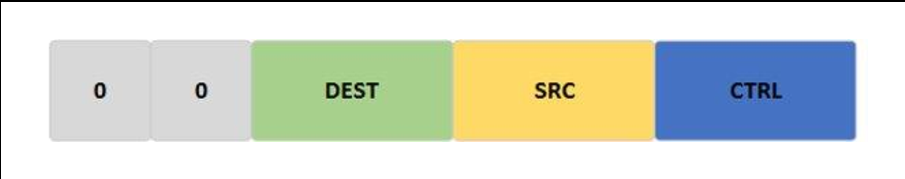
\includegraphics[width=\textwidth]{figures/ControlPacket.pdf}
    \caption{Composition of a control packet}\label{fig:ControlPacket}
\end{figure}

A control packet is indicated by two leading zeroes. Followed by source address (2 bits) and destination address (2 bits).

\section{Bus monitor}

How is it set up?

Made assumptions?

Document used / invented protocol.

